% Done: PdBI observations, VLA observations
%
%
%
%
%


\documentclass[]{emulateapj}
\usepackage{amsmath}

\usepackage[breaklinks,colorlinks,citecolor=blue,linkcolor=blue]{hyperref}
\usepackage{etoolbox}

\makeatletter

% Patch case where name and year are separated by aysep
\patchcmd{\NAT@citex}
  {\@citea\NAT@hyper@{%
     \NAT@nmfmt{\NAT@nm}%
     \hyper@natlinkbreak{\NAT@aysep\NAT@spacechar}{\@citeb\@extra@b@citeb}%
     \NAT@date}}
  {\@citea\NAT@nmfmt{\NAT@nm}%
   \NAT@aysep\NAT@spacechar\NAT@hyper@{\NAT@date}}{}{}

% Patch case where name and year are separated by opening bracket
\patchcmd{\NAT@citex}
  {\@citea\NAT@hyper@{%
     \NAT@nmfmt{\NAT@nm}%
     \hyper@natlinkbreak{\NAT@spacechar\NAT@@open\if*#1*\else#1\NAT@spacechar\fi}%
       {\@citeb\@extra@b@citeb}%
     \NAT@date}}
  {\@citea\NAT@nmfmt{\NAT@nm}%
   \NAT@spacechar\NAT@@open\if*#1*\else#1\NAT@spacechar\fi\NAT@hyper@{\NAT@date}}
  {}{}
  
\makeatother
%
\usepackage{xspace}
%
\usepackage{apjfonts}
\usepackage{amssymb, amsmath} % for e.g. \lesssim
\usepackage{natbibspacing, natbib}
\usepackage{aas_macros} % for understanding Journal in bib
\usepackage{graphics,graphicx}
%
\newcommand{\vdag}{(v)^\dagger}
\newcommand{\myemail}{tleung@astro.cornell.edu}
\newcommand{\Msun}{\mbox{$M_{\odot}$}\xspace}
\newcommand{\Rsun}{\mbox{$R_{\odot}$}\xspace}
\newcommand{\Lsun}{\mbox{$L_{\odot}$}\xspace}
\newcommand{\LIR}{\mbox{$L_{\rm IR}$}\xspace}
\newcommand{\LFIR}{\mbox{$L_{\rm FIR}$}\xspace}
%
\newcommand{\rarr}{$\rightarrow$}
\newcommand{\aco}{\mbox{CO($J$\,=\,1\,\rarr\,0) }}
\newcommand{\bco}{\mbox{CO($J$\,=\,2\,\rarr\,1) }}
\newcommand{\cco}{\mbox{CO($J$\,=\,3\,\rarr\,2) }}
\newcommand{\rot}[3][CO]{\mbox{#1($J$\,=\,#2\,\rarr\,#3)}}
%
\newcommand{\cii}{[C{\scriptsize II}]}
\newcommand{\Lp}[1][CO]{\mbox{$L^{\prime}_\textrm{\fontsize{8pt}{12pt}\selectfont{#1}}$}\xspace}
\newcommand{\kms}{\mbox{km\,s$^{-1}$}\xspace}
\newcommand{\LpU}{\mbox{K\,\,km\,\,s$^{-1}$\,\,pc$^2$}\xspace}
\newcommand{\pmOne}{\mbox{$^{-1}$}\xspace}
\newcommand{\alphaco}{\mbox{$\alpha_{\rm CO}$}\xspace}
\newcommand{\alphaU}{\mbox{$($K\,\,\kms\,\,pc$^2$$)$\pmOne}}
\newcommand{\sfrU}{\mbox{\Msun\,yr$^{-1}$}\xspace}
% Numerical values
\newcommand{\E}[1]{\mbox{$\times10^{#1}$}}
\newcommand{\petm}[2]{$^{+#1}_{-#2}$}
\newcommand{\eq}{\,=\,}
\newcommand{\pmm}{\,$\pm$\,}
%
\newcommand{\eg}{{e.g.,~}}
\newcommand{\ie}{{i.e.,~}}
%
\newcommand{\Fig}[1]{Figure~\ref{fig:#1}}
\newcommand{\Eq}[1]{Equation~\ref{eq:#1}}
\newcommand{\Tab}[1]{Table~\ref{tab:#1}}
\newcommand{\Sec}[1]{\S\ref{sec:#1}}
%
\newcommand\tna{\,\tablenotemark{a}}
\newcommand\tnb{\,\tablenotemark{b}}
\newcommand\tnc{\,\tablenotemark{c}}
\newcommand\tnd{\,\tablenotemark{d}}
\newcommand\tne{\,\tablenotemark{e}}
\newcommand\tnf{\,\tablenotemark{f}}
\newcommand\tng{\,\tablenotemark{g}}
\newcommand\tnh{\,\tablenotemark{h}}
\newcommand\tni{\,\tablenotemark{i}}
\newcommand\tnj{\,\tablenotemark{j}}
\newcommand\tnk{\,\tablenotemark{k}}
\newcommand\tnl{\,\tablenotemark{l}}
%
\def\herschel {{\it Herschel Space Observatory}\xspace}
\def\alma     {Atacama Large (sub-)Millimeter Array (ALMA)\xspace}
\def\spitzer {{\it Spitzer Space Telescope}\xspace}
\def\pdbi     {Plateau de Bure Interferometer\xspace}
\def\carma    {Combined Array for Research in Millimeter-wave Astronomy\xspace}
\def\cso      {Caltech Sumillimeter Observatory (CSO)\xspace}
\def\noema    {Northern Extended Millimeter Array (NOEMA)\xspace}
\def\vla      {{\it Karl G. Jansky} Very Large Array\xspace}
% Typography
\newcommand{\ncode}[1]{{\sc #1}}
% Codes / Softwares
\newcommand{\uvmcmcfit}{\ncode{uvmcmcfit}\xspace}
\def\aips {\ncode{AIPS}\xspace}
\def\casa {\ncode{CASA}\xspace}
% Long words
\newcommand{\lowZ}{low-metallicity\xspace}
\newcommand{\mulw}{multi-wavelength\xspace}
\newcommand{\SF}{star formation\xspace}
\newcommand{\SB}{starburst\xspace}
\newcommand{\SBs}{starbursts\xspace}
\newcommand{\gl}{gravitationally lensed\xspace}
\newcommand{\MCMC}{Markov Chain Monte Carlo (MCMC)\xspace}
% Wavelength regimes
\newcommand{\fir}{far-IR\xspace}
\newcommand{\fuv}{far-UV\xspace}
\newcommand{\mir}{mid-IR\xspace}
\newcommand{\nir}{near-IR\xspace}
\slugcomment{To be submitted to the ApJ}

\citestyle{aa}
\shorttitle{Something goes here}
\shortauthors{Leung \& Riechers}

\begin{document}
%{\tiny  \RevisionInfo}

\title{Gas Dynamics of the Einstein ring RXSJ1131-1123 at $z$=0.654}
\author{T. K. Daisy Leung and Dominik A. Riechers}
\affil{Department of Astronomy, Space Sciences Building, Cornell University,
Ithaca, NY 14853, USA; \myemail}
%==============================================================================
%                                Front matters
%==============================================================================

\begin{abstract}
\end{abstract}

\keywords{ISM: molecular --
          infrared: galaxies --
          galaxies: starburst --
          galaxies: evolution}

%--------------------------------------------------------------------------
%                                Introduction
%--------------------------------------------------------------------------
\section{Introduction}

%--------------------------------------------------------------------------
%                          Observations details
%--------------------------------------------------------------------------
\section{Observations}
\subsection{PdBI \bco} % DONE
Observations of the \bco rotational line ($\nu_{\rm rest}$ = 230.5379938 GHz)
toward the \gl galaxy RXJ1131-1231 at $z_{\rm QSO}$ =
0.658 were carried out using IRAM \pdbi (PdBI; Program ID: S14BX001; PI: D.
Riechers). Two observing runs were carried out on 2014 December 06 and 2015
February 05 under good weather conditions in the C and D array configurations,
respectively. The 2 mm receivers were used to cover the redshifted \bco line
and the underlying continuum emission, employing a correlator setup providing
an effective bandwidth of 3.6 GHz and a spectral resolution of 10.0 MHz ($\sim$
21.5 \kms). This resulted in 3.75 hours of cumulative six antenna-equivalent on
-source time after discarding unusable visibility data.
The nearby quasars 1127$-$145 and 1124$-$186 were observed every 22 minutes
for pointing, secondary amplitude, and phase calibration and 1055$+$018 was
observed as bandpass calibrators for both tracks.
MWC349 and 3C279 were observed as the primary flux calibrator for C and D
array observations, respectively, yielding $\lesssim$15\% calibration accuracy.

The \ncode{GILDAS} package was used to reduce and analyze the visibility data
which are then imaged and deconvolved using the CLEAN algorithm with ``natural"
weighting. This yields a synthesized clean beam size of 4$\farcs$44 $\times$ 1\farcs95 (PA = 13\degr). The final rms noise is $\sigma$ = 0.177 Jy \kms beam\pmOne over a channel width of 320 MHz (690 \kms), and $\sigma$ = 1.451 mJy \kms
beam\pmOne over 10 MHz (21.5 \kms). The continuum image at $\nu_{\rm cont}\sim$
139 GHz is created by averaging over all the line-free channels. This
yields an rms noise of 0.082 mJy beam$^{-1}$. % see README.md in 04Sep15

\subsection{CARMA \cco}
% 1127-189 Gain for set 2
% 3C273 gain for set 3
% after flagging: Total observing time is  1.48 hours, checked with uvindex for
% set 3
% after flagging: Total obs. time is 2.94 hours, checked with uvindex for the
% combined set
% 12.500 MHz <=> 17.935 km/s
Observations of the \cco rotational line ($\nu_{\rm rest}$ = 345.7959899 GHz)
were carried out under the D array configurations of the \carma (CARMA;
Program ID: cf0098; PI: D. Riechers) on 2014 February 02 under terrible 3\,mm
weather conditions and on 2014 February 17 under good 3\,mm
weather conditions. The correlator setup provides a bandwidth of 3.75 GHz in
each sideband and a spectral resolution of 12.5 MHz ($\sim$17.9 \kms). The
line was placed in the lower sideband with the local oscillator tuned to $\nu_{\rm LO}\sim$216 GHz. The radio quasars J1127$-$189 (first track) and 3C273 (
second track) were observed
every 15 minutes for pointing, amplitude, and phase calibration. Mars was
observed as the primary absolute flux calibrator and 3C279 was observed as
bandpass calibrators for both tracks. This results in a total on-source time of 2.94 hours after flagging poor
visibility data.

% poor phase note
Given that the phase calibrator used for the first track was faint and was
observed under poor weather conditions and that the phase calibrator used for
the second track was far from our target source, the phase calibration is
subpar, with an rms scatter $\sim$60\degr. We thus conservatively estimate
a calibration accuracy of $\sim$BLAH\% based on the flux scale uncertainties,
gain variation over time, and the phase scatter on the calibrated data. We
therefore treat its line intensity and refrain using it to derive other physical quantities.

The \ncode{MIRIAD} package was used to calibrate the visibility data which are
then imaged and deconvolved using the CLEAN algorithm with ``natural" weighting. This yields a synthesized clean
beam size of 3\farcs2 $\times$ 1\farcs9 (PA = 8\degr) for the lower sideband
image cube. The final rms noise is $\sigma$ = 13.3 mJy km s$^{-1}$ beam$^{-1}$
over a channel width of 25 MHz.

\subsection{VLA} %DONE
Our analysis also use the archival data of the radio continuum obtained with the \vla (VLA; Program ID: AW741; PI: Wucknitz). Since these data have not been
published, we here describe the details of the observations as well as our calibration steps.

Observations were carried out on 2008 December 29 under excellent weather
conditions in the A array configurations for a total of $\sim$7 hours on-source time. The C-Band receivers were used with a continuum mode setup, providing a bandwidth of 50
MHz in each sideband.
The nearby radio quasar 1130$-$149 was observed every 10 minutes for
pointing, amplitude, and phase calibration, 1331$-$305 was observed as the
primary flux calibrator, and 0319$+$415 was observed as the bandpass calibrator, yielding $\sim$15\% calibration accuracy.
We use \aips to calibrate the visibility data which
are then imaged and deconvolved using
the CLEAN algorithm using robust\,=\,0. This yields a synthesized clean
beam size of 0$\farcs$49 $\times$ 0\farcs35 (PA\,=\, 0\farcs18) and a final
rms noise of $\sigma$ = 13 $\mu$Jy beam\pmOne.


\section{HST astrometry}
We gathered optical (rest-frame UV) images for RXJ1131 from the Hubble Legacy Archive to illustrate the
spatial extent of different emission detected in this paper. Here, we only use the F555W image for
this purpose.
We adopt the VLA 5\,GHz map of $\sim$2" resolution as the reference coordinate frame to align the optical image.
We shifted the latter to the east by 0\farcs5963 in R.A. and +0\farcs8372 in Dec., which is consistent with the typical astrometric precision of the HST image from the Hubble
Legacy Archive. % for Hubble Legacy Archive: abs. astronmetry 1-2" http://hla.stsci.edu/hla_faq.html
The radio image is calibrated employing well-monitored phase calibrator, with positions known to $\sim$1 mas.
We estimate the absolute alignment of the 5 GHz and CO(J=2-1) coordinate frames should
be better than 0.1", leaving aside uncertainties relating to the SNR and beam size.


%The astrometry of the HST images was firstly calibrated against a wider-field
%optical image of the cluster which had in turn been aligned onto the FK5
%coordinate system to an rms precision of ~0.2".

%--------------------------------------------------------------------------
%                                Results
%--------------------------------------------------------------------------
\section{Results}
\subsection{\bco}
\subsection{\cco}
\subsection{Interferometric Continuum}
2mm: resolved along the major axis, but unresolved along the minor axis. We decomposed the continuum from the foreground and background sources by subtracting a point
source model in the uv-plane (see Riechers+13 SMMJ04135 description)


\subsection{Photometry from archive}
We obtain archival and published photometry.
2MASS magnitudes from the 2MASS All-Sky
Catalog of Point SourcesBLAH  (Skrutskie et al. 2006), WISE magnitudes
from the AllWISE Source CatalogBLAH, Spitzer/MIPS
data from BLAH Catalog, IRAS photometry from the IRAS point source
and faint source cataloguesBLAH.

The Herschel/SPIRE data are from the Herschel Science Archive, processed
by the SPIRE HIPE pipeline version 12BLAH (Ott 2010). The
photometry was extracted at the source position using the
SUSSEXTractor task within HIPE (Savage \& Oliver 2007,
Smith et al 2012, Pearson et al 2014). The SUSSEXtractor
task estimates the flux density from an image smoothed with
a convolution kernel derived from the SPIRE beam FWHM.
The flux density measured by SUSSEXtractor
was verified using the SPIRE Timeline Fitter (Bendo et
al. 2013) which fits a two dimensional elliptical Gaussian
function at the source position in the timeline data. The
agreement between the SUSSEXtractor and Timeline Fitter
flux densities was found to be better than $\sim$BLAH per cent.

We list the mid-IR to FIR photometries compiled from 2MASS, WISE,IRAS, IRAC catalogs in \Tab{photometry}.
\begin{deluxetable}{lccc}[tbpH]
\tabletypesize{\scriptsize}
\tablecolumns{4}
\tablecaption{Photometry data}
\tablehead{\colhead{Wavelength } & \colhead{Frequency } & \colhead{Flux Density } & \colhead{Instrument}\\ \colhead{micron} & \colhead{GHz} & \colhead{mJy} & \colhead{ }}
\startdata
0.555 & 540167.0 & 0.056 $\pm$ 0.006 & HST-ACS/V-Band(L) \\
0.555 & 540167.0 & 0.009 $\pm$ 0.0041 & HST-ACS/V-Band(H) \\
0.814 & 368295.0 & 0.238 $\pm$ 0.013 & HST-ACS/I-Band(L) \\
0.814 & 368295.0 & 0.041 $\pm$ 0.0054 & HST-ACS/I-Band(H) \\
1.25 & 239834.0 & 1.009 $\pm$ 0.09 & 2MASS/J-Band \\
1.6 & 187370.0 & 0.539 $\pm$ 0.041 & HST-NICMOS(NIC2)/H-Band(L) \\
1.6 & 187370.0 & 0.133 $\pm$ 0.004 & HST-NICMOS(NIC2)/H-Band(H) \\
1.65 & 181692.0 & 1.448 $\pm$ 0.12 & 2MASS/H-Band \\
2.17 & 138153.0 & 2.064 $\pm$ 0.16 & 2MASS/Ks-Band \\
3.4 & 88174.2 & 7.027 $\pm$ 0.14 & WISE/W1 \\
3.6 & 83275.7 & 5.618 $\pm$ 0.0021 & Spitzer/IRAC(Extracted) \\
3.6 & 83275.7 & 5.034 $\pm$ 0.0021 & Spitzer/IRAC(Host) \\
3.6 & 83275.7 & 0.585 $\pm$ 0.003 & Spitzer/IRAC(Archive-Host) \\
4.5 & 66620.5 & 7.803 $\pm$ 0.0021 & Spitzer/IRAC(Archive) \\
4.5 & 66620.5 & 6.009 $\pm$ 0.0017 & Spitzer/IRAC(Host) \\
4.5 & 66620.5 & 1.794 $\pm$ 0.0027 & Spitzer/IRAC(Archive-Host) \\
4.6 & 65172.3 & 8.872 $\pm$ 0.16 & WISE/W2 \\
5.8 & 51688.4 & 10.720 $\pm$ 0.0051 & Spitzer/IRAC(Archive) \\
5.8 & 51688.4 & 7.557 $\pm$ 0.003 & Spitzer/IRAC(Host) \\
5.8 & 51688.4 & 3.163 $\pm$ 0.0059 & Spitzer/IRAC(Archive-Host) \\
8.0 & 37474.1 & 14.470 $\pm$ 0.0041 & Spitzer/IRAC(Archive) \\
8.0 & 37474.1 & 9.881 $\pm$ 0.0039 & Spitzer/IRAC(Host) \\
8.0 & 37474.1 & 4.589 $\pm$ 0.0057 & Spitzer/IRAC(Archive-Host) \\
12.0 & 24982.7 & 21.960 $\pm$ 0.42 & WISE/W3 \\
12.0 & 24982.7 & 400.000 $\pm$ \nodata & IRAS \\
22.0 & 13626.9 & 55.110 $\pm$ 1.9 & WISE/W4 \\
24.0 & 12491.4 & 47.180 $\pm$ 0.026 & Spitzer/MIPS \\
25.0 & 11991.7 & 500.000 $\pm$ \nodata & IRAS \\
60.0 & 4996.54 & 600.000 $\pm$ \nodata & IRAS \\
100.0 & 2997.92 & 1000.000 $\pm$ \nodata & IRAS \\
250.0 & 1199.17 & 289.427 $\pm$ 9.6 & Herschel/SPIRE \\
350.0 & 856.55 & 168.229 $\pm$ 8.6 & Herschel/SPIRE \\
500.0 & 599.585 & 56.782 $\pm$ 8.8 & Herschel/SPIRE \\
1387.93 & 216.0 & 2.492 $\pm$ \nodata & CARMA \\
2152.82 & 139.256 & 1.230 $\pm$ 0.22 & PdBI-integrated \\
2152.82 & 139.256 & 0.799 $\pm$ 0.082 & PdBI-peak \\
2152.82 & 139.256 & 0.400 $\pm$ 0.082 & PdBI-removedFG \\
61414.0 & 4.8815 & 1.273 $\pm$ 0.042 & VLA/Cband-arc \\
61414.0 & 4.8815 & 0.866 $\pm$ 0.027 & VLA/Cband-core
\enddata
\label{tab:BLAH}
\tablecomments{blah}
 %TablenotegoesBetween 
\tablerefs{blah}
\end{deluxetable}

%--------------------------------------------------------------------------
%                                Analysis
%--------------------------------------------------------------------------
\section{Analysis}
\subsection{Lens modeling}
With the high SNR and spectral resolution, we model different kinematic components using our lensing code \uvmcmcfit.

% describe model setup.


% comparison with C06 model


\begin{figure*}[tbph]
\centering
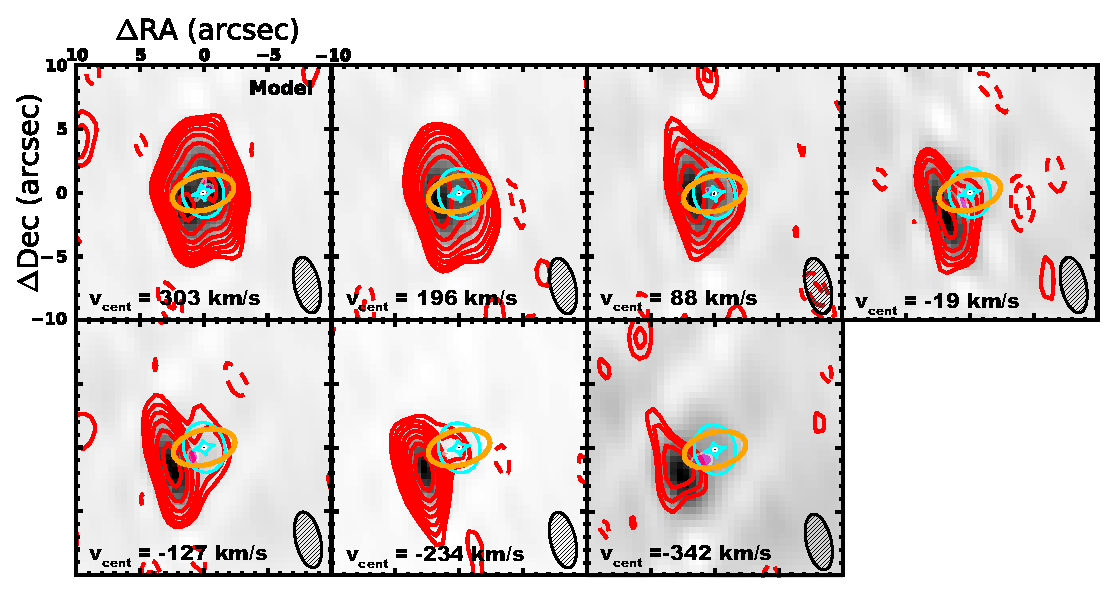
\includegraphics[width=0.85\textwidth]{../Figures/PostageStampModel.eps}
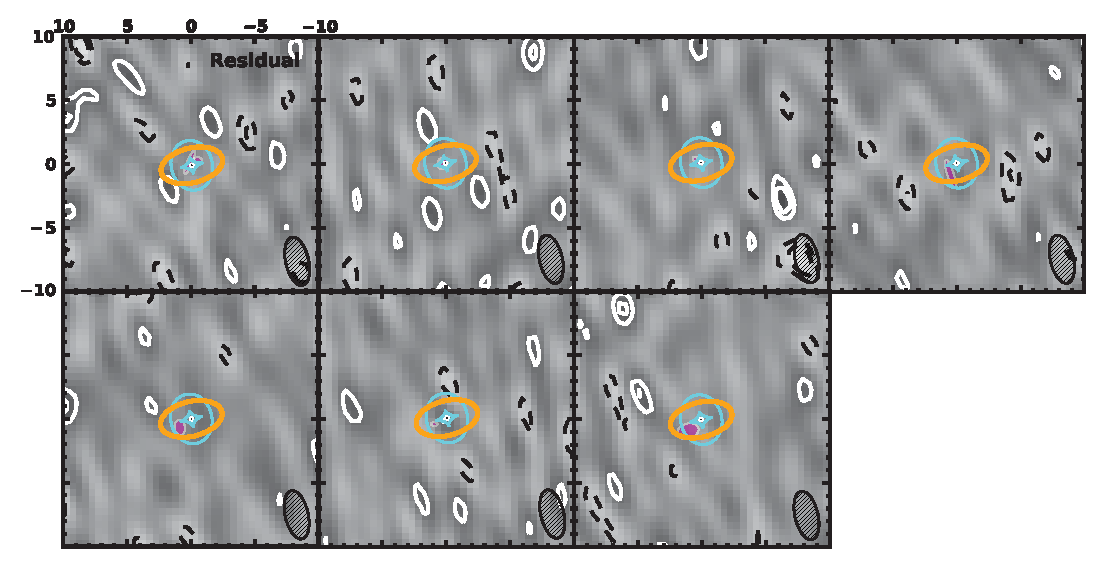
\includegraphics[width=0.85\textwidth]{../Figures/PostageStampResiduals.eps}
\caption{
Lens model of channel widths $\sim$ 100\kms.
Make this bigger in the future
\label{fig:}}
\end{figure*}



\subsubsection{Differential Lensing}
Lens modeling of this source from previous studies find non-negligible differential lensing effect across H-Band, V-band, and I-band. The magnification factor ranges from 10.9
to 7.8, where the decrease is caused
by the more extended IR emission (hence SF), well beyond the caustic (C06).

The highly asymmetric \bco line profile also suggests that differential lensing is non-negligible in the CO emission, where
flux density in the red wing is apparently much higher than in the blue wing, given its lensing configuration.
By modeling different kinematic components, we find that the magnification factor ranges from BLAH to BLAH. The various magnification factors are listed in Table \ref{tab:}.
\begin{deluxetable}{lcc}[!htbp]
\tabletypesize{\scriptsize}
\tablecolumns{3}
\tablecaption{Magnification factors of various kinematic components in \bco}
\tablehead{
\colhead{Velocity Range(\kms)} & % see 22May16/intensity30Apr16.spec; or channel map in paper
\colhead{Source 1 $\mu_{\rm L}$} &
\colhead{Source 2 $\mu_{\rm L}$}
}
\startdata
$-$366\,$-$\,$-$258 & 3.1 $\pm$ 0.9 & \\ [0.5ex]
$-$237\,$-$\,$-$151 & 4.3 $\pm$ 2.4 & \\ [0.5ex]
$-$129\,$-$\,$-$43  & 4.2 $\pm$ 0.6 & \\ [0.5ex]
$-$21.5\,$-$\,65    & 4.1 $\pm$ 0.9 & \\ [0.5ex]
86\,$-$\,172        & 8.7 $\pm$ 2.0 & \\ [0.5ex]
194\,$-$\,280       & 7.6 $\pm$ 1.6 & \\ [0.5ex]
301\,$-$\,388       & 7.2 $\pm$ 5.6 & 6.7 $\pm$ 2.5 \\ [0.5ex]
weighted average & 4.4 & \\ [0.5ex]
median & 5.5 &
\enddata
\label{tab:model}
\tablecomments{Velocity is taken from the center of each (native) channel
without any binning. Each row corresponds to a channel slice used for
lens modeling. Source 1 is RXJ1131 and source 2 is its companion. See text for details. }
\end{deluxetable}




\subsection{\bco Dynamical modeling}
Based on the the source plane position of each kinematic components from the
lens model, a clear symmetric velocity gradient is seen, which is suggestive of a rotating disk. Assuming the observed velocities of the respective channels
correspond to solely the tangential components (i.e. $\theta$ = 0), we extract
the major axis along the best-fit slice across these source plane positions,
which is along PA of 121\degr.
We attempt to characterize the molecular gas kinematics using an empirically motivated disk model (e.g. Courteau97, Peuch+08, Miller+11):
\begin{equation}
V = V_0 + \frac{2}{\pi} V_a arctan(\frac{R}{R_t}),
\end{equation}
where $V$ is the observed velocity, $V_0$ is the velocity at dynamical center, $V_a$ is the asymptotic velocity, and $R_t$ is the ``turnover'' radius at which the rotation curve
becomes flat. We perform non-linear least square fitting using an orthogonal distance regression to find the best-fit $V_a$, $r_t$, $V_0$, taking into account
errors in both velocity and distance offset (see Figure \ref{fig:PV}). We also place an upper limit on $r_t$ $<$ 15 kpc (Miller+11, Genzel+??, Puech+08?) to keep this
parameter physical. We then estimate the uncertainties associated with best-fit parameters using a Monte Carlo simulation of 500 iterations, perturbing
the velocity and physical separation according to a random Gaussian distribution of width based on the input uncertainties on
the data. Using this model, we find $V_a$ = 975$\pm$387, $r_t$ = 10.6$\pm$5.7,
and $V_0$ = 28$\pm$40. We note, however, that since emission is not detected beyond the flat regime of the rotation curve (Figure \ref{fig: PV}), the asymptotic velocity is
poorly constrained. In particular, $V_a$ and $r_t$ are highly correlated with a Pearson coefficient $r$ = 0.998 between the two, and 0.027 between $V_a$ and $V_0$.

While a symmetric velocity field in the source plane is consistent with a rotating disc, such is insufficient to conclude a rotating disk morphology. Additional characteristics such
as peak velocity dispersion at the center of a galaxy and a ``spider'' diagram are needed. Based on the reconstructed source plane in the optical/NIR emission, C06 find that a
n=1 Sersic profile is best

The frequently used Vmax (maximum measured velocity) is not equivalent to the
asymptotic value, Va, a mathematical extrapolation and typically not reached in
the observed rotation curve. Estimates of Va can depend critically on how well
the central region and turn over of the rotation curve are constrained. For the
remaining analysis, we adopt the asymptotic limit as a proxy to the rotation
curve. We also note that typical studies of the Tully-Fisher relation uses V_2.2
(2.2 * disc scalelength ~ 1.375 half-light radius ~ 0.7R_opt) as the rotation
velocity since this would be the radius at which the velocity of a pure
exponential disc peaks at. However, our source appears to be a disturbed
rotator, albeit coarse resolution. Hence, rather than adopting V_2.2, we use the
asymptotic value from the best-fit arctangent model. The half light radius in the
optical is ~xx kpc (from C06; converted in to our cosmology, but BJB 8 kpc
across?).


If we adopt the best-fit parameters, we find a dynamical mass of $M_{\rm dyn}$($<$blah kpc) sin$^2 i$ = BLAH \Msun. Consider the line widths using the separation between
the red- and blue- shifted emission of the \bco line profile of $\Delta v_{\rm sep}/2 \sim$ blah \kms and a source size of blah kpc, we find a dynamical mass of $M_{\rm dyn}$
sin$^2 i$ = BLAH \Msun. If we adopt the inclination angle using the morphological axis ratio from the
reconstructed optical image reported by C06, where the minor axis is 1\farcs8 and the major axis is 3\farcs3.25, then we find an inclination angle of 56.4
\degr. Then $M_{\rm dyn}$\,=\,BLAH. The inclination angle is consistent with the observed unobscured AGN and an observable double peak line profile.

We note, however, that large differences (up to $\gtrsim$10 deg) can be found between such kinematically-derived inclinations and the ones inferred from the morphological
axis ratio (e.g., Chemin et al. 2006). We caution that this analysis is based on limited spatial resolution data and will been verified by future higher-resolution observations.

\subsection{SED modeling}
\subsection{ISM properties}
\subsection{Gas Mass}
\subsection{Source Extent}
Compared to HST:

%--------------------------------------------------------------------------
%                                Discussion
%--------------------------------------------------------------------------
\section{Discussion}
\subsection{At what stage is the merging in RXJ1131-1231?}



\subsection{Implications} gas fraction at this redshift. how does that relate to
the SFH. --> imply the change in cosmic SFD is due to change in gas content. SFE
at this redshift, how does that relate to the SFH. probably a secondary effect
to the drop in SFH


  %--------------------------------------------------------------------------
%                                Conclusions
%--------------------------------------------------------------------------
\section{Summary and Conclusions}
We studied a wet-wet merger between a AGN/starburst ULIRG and a optically faint companion at $z$ $\sim$ 0.65.





%==============================================================================
%                                Back matters
%==============================================================================


% ACKNOWLEDGEMENTS
%-----------------
\acknowledgments


  %--------------------------------------------------------------------------
  %                               Bibliography
  %--------------------------------------------------------------------------
\bibliographystyle{yahapj}
\bibliography{RXJ.bib}
\end{document}